\part{Deep learning}
\frame{\partpage}

\begin{frame}{Deep learning}
	\begin{itemize}
		\pause\item Basically, the use of large ANNs with \textbf{many layers}
		\pause\item Often uses \textbf{large training sets}
		\pause\item Training often uses powerful \textbf{GPUs} --- many times faster than training on the CPU
	\end{itemize}
\end{frame}

\begin{frame}{Convolutional Neural Networks (ConvNets)}
	\begin{center}
		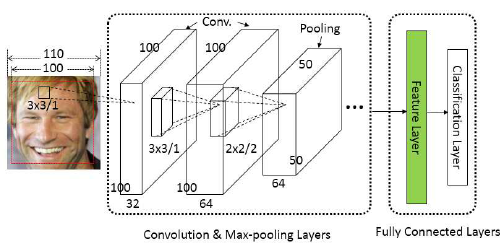
\includegraphics[width=0.5\textwidth]{convnet}
	\end{center}
	\begin{itemize}
		\pause\item Layers are \textbf{2D arrays}
		\pause\item Neurons in convolutional layers are only connected to nearby neurons
		\pause\item There are also fully connected layers
	\end{itemize}
\end{frame}

\begin{frame}
	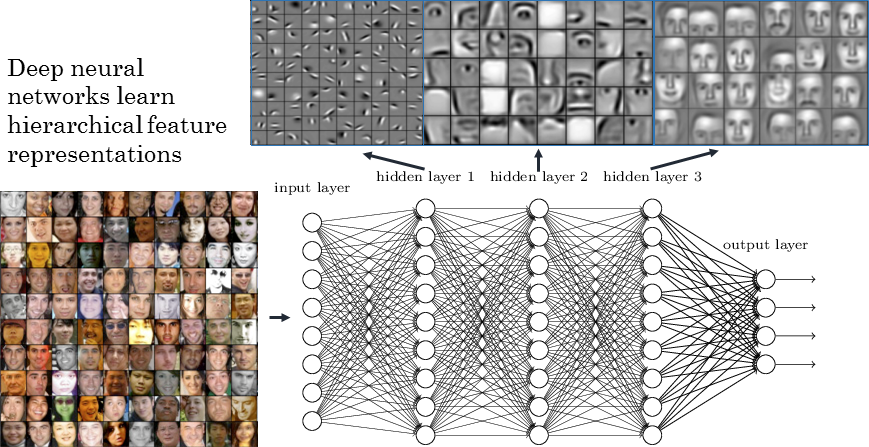
\includegraphics[width=\textwidth]{convnet_face}
\end{frame}

\begin{frame}{DeepDream}
	\begin{itemize}
		\pause\item Train a ConvNet to recognise something (e.g.\ faces, objects, animals)
		\pause\item Run the network in ``reverse''
			\begin{itemize}
				\pause\item Adjust the image (e.g.\ via gradient ascent) so that it is more strongly recognised by the network
			\end{itemize}
	\end{itemize}
\end{frame}

\begin{frame}{DeepDream}
	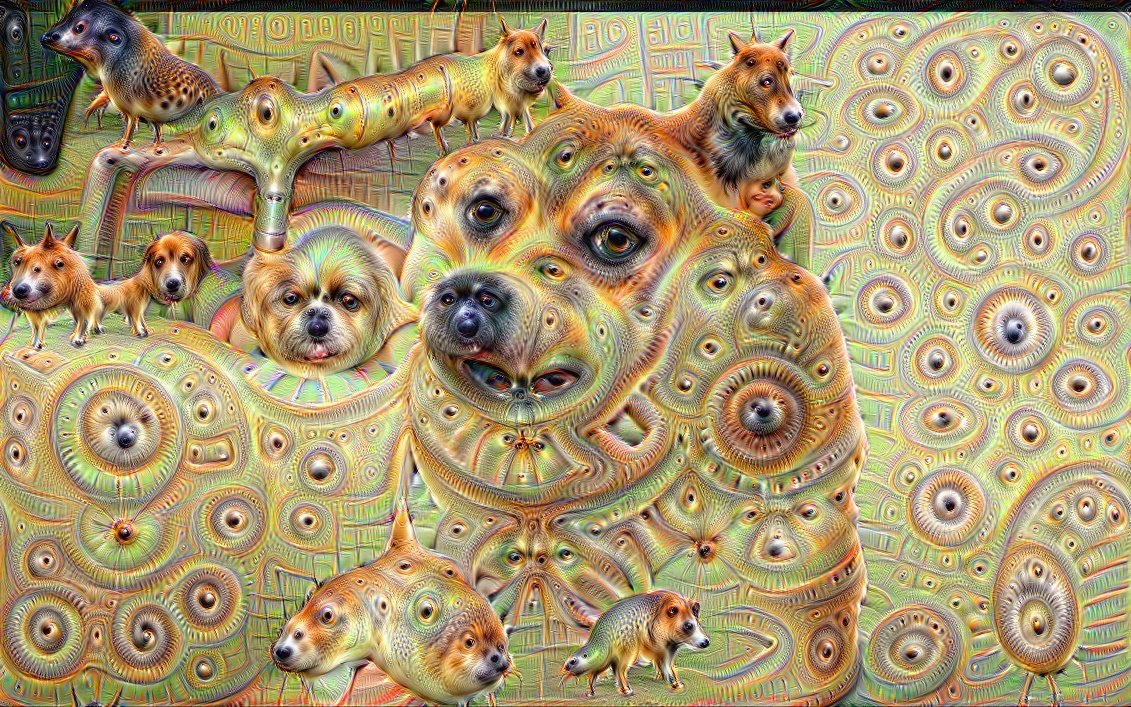
\includegraphics[width=\textwidth]{deepdream}
\end{frame}

\begin{frame}{Style transfer}
	\begin{itemize}
		\pause\item Train a ConvNet to recognise a particular artistic style
		\pause\item Run the network in ``reverse'' on an input image
			\begin{itemize}
				\pause\item Adjust the image (e.g.\ via gradient ascent) so that it is more strongly recognised by the network
			\end{itemize}
	\end{itemize}
\end{frame}

\begin{frame}
	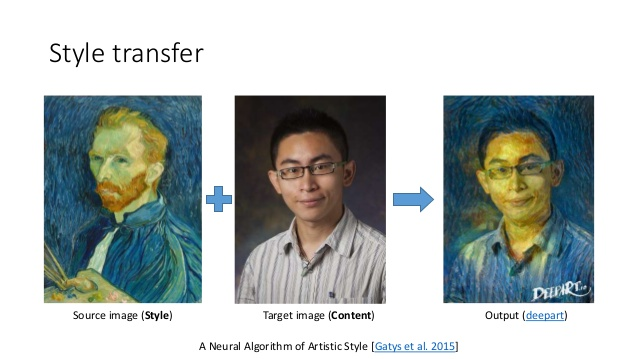
\includegraphics[width=\textwidth]{style_transfer}
\end{frame}

\begin{frame}{Learning to play Atari games (Mnih et al, 2015)}
	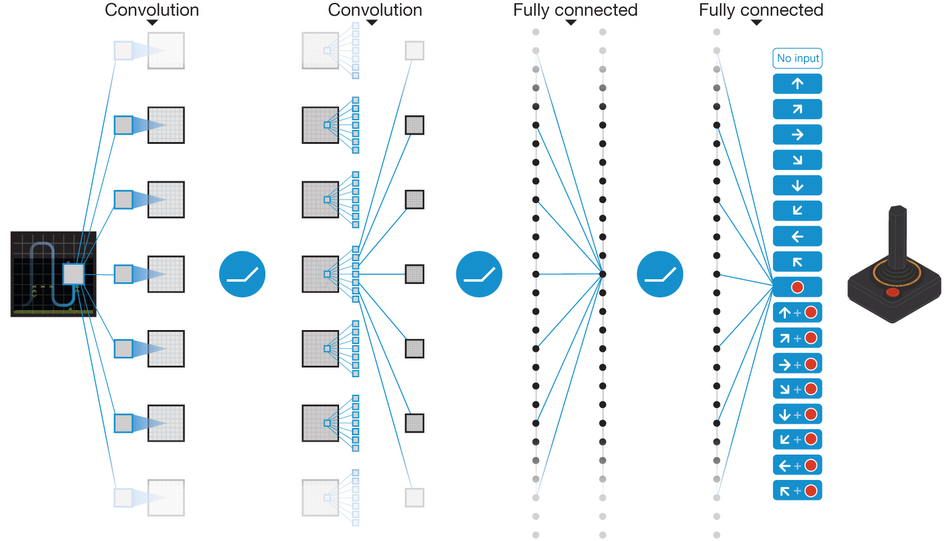
\includegraphics[width=\textwidth]{deepmind_atari}
\end{frame}

